\section{Processing System Mass}
The function of the processing system is to receive asteroid material from the excavation system and process it into pure water.
At the time of writing this, there is no system within the model that purifies the water, it is therefore assumed the output of initial processing is pure water. This is likely an invalid assumption that needs to be corrected.
The main components of the processing system are a container to house the asteroid material and a power source to convert the asteroid material into water. The processing container volume is given by:
\begin{equation}
    V_{processing} = V_{excavation} / n_{processingNumberBatches}
\end{equation}
\begin{equation}
    m_{asteroidProcessing} = V_{processing} / density_{asteroid}
\end{equation}
as there is no need for the processing system to work on the same mass scale as the excavation system. The Processing container mass is calculated the same as the excavation container mass using equations 4-6. There are separate parameters for each system in the model to decouple the excavation system design from the processing system design. Additionally, in some architectures the processing could be done in the excavation container. This can easily be accomplished by setting the processing material density to 0.
\newline
The bulk of the processing system mass comes from the power needed to transform the asteroid material into water. The dehydration reaction takes place at 600C. All power and energy calculations are done on a per batch basis.
\begin{equation}
    E_{thermal} = Cp_{asteroid} \cdot (T_{end} - T_{start}) \cdot m_{asteroidProcessing}
\end{equation}
\begin{equation}
    E_{reaction} = H_{reaction} \cdot frac{m_{asteroidProcessing} / x_{asteroidWaterPercent}}{0.01802} 
\end{equation}
\begin{equation}
    E_{total} = E_{thermal} + E_{reaction}
\end{equation}
The total power of the system is calculated by dividing the total energy by the processing time. The processing time, in days, is an input to the model.
\begin{equation}
    P_{batch} = E_{total} / t_{processing} \cdot (1/24)(1/60)(1/60)
\end{equation}
Since the model uses processing time as an input, the design confirms to meet the specified processing times. Therefore, the time should be consistent no matter the amount of water being harvested. This is shown and confirmed in \autoref{fig-processTime}
\begin{figure}[htb]
    \centering
    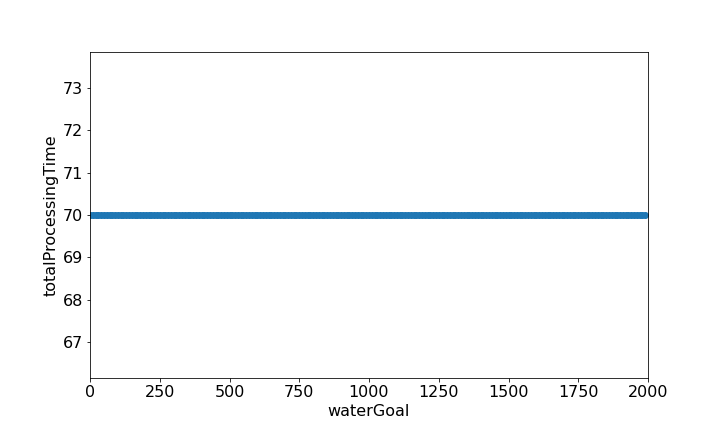
\includegraphics[width=0.5\linewidth]{processTime_vs_waterGoal.png}
    \captionsetup{justification=centering,margin=2cm}
    \caption{Processing time (days) over a range of water targets. The model treats processing time as an input variable, so the constant nature of this graph is expected}
    \label{fig-processTime}
\end{figure}


The total energy required for the processing system is shown in \autoref{fig-processingEnergy}.
\begin{figure}[htb]
    \centering
    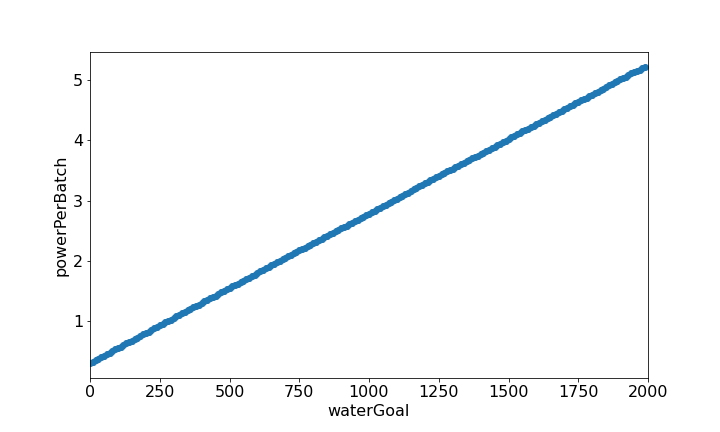
\includegraphics[width=0.5\linewidth]{powerPerBatch_vs_waterGoal.png}
    \caption{Processing energy (kW) per batch for a range of water targets (kg). }
    \captionsetup{justification=centering,margin=2cm}
    \label{fig-processingEnergy}
\end{figure}

The energy can come from two different ways: solar thermal power or through converting electricity to heat. The base assumption in the model is that solar panels will be used to produce electricity, and that will be turned into heat energy for processing the asteroid material. The energy density inputs can be easily changed to assess a different energy source, such as solar thermal concentrators. 
\begin{equation}
    m_{solarPanels} = \frac{P_{batch}}{SolarPanel_{EnergyDensity}\cdot e_{electricityToHeat} \cdot \frac{1}{r_{asteroidToSun}^2} \cdot (1 - SolarPanel_{degradation})^{designYears}}  
\end{equation}

The total processing mass is given by:
\begin{equation}
    m_{processing} = m_{container} \cdot containerMass_{factor} + m_{solarPanels} 
\end{equation}
\begin{figure}[htb]
    \centering
    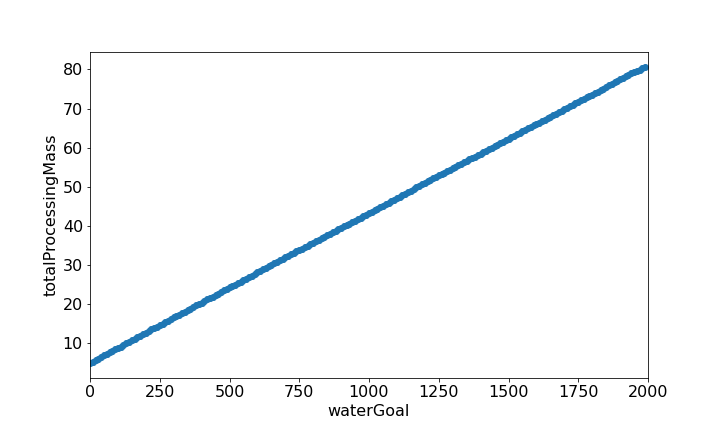
\includegraphics[width=0.5\linewidth]{processMass_vs_waterGoal.png}
    \captionsetup{justification=centering,margin=2cm}
    \caption{Processing mass (kg) over a range of water targets. Both values are in kilograms.}
    \label{fig-processMass}
\end{figure}
